\documentclass[aspectratio=169, table, 12pt]{beamer}

\usepackage{colortbl}
\usepackage{xcolor}
\usepackage{listings}
\usepackage{tabularx}
\usepackage{tikz}
\usetikzlibrary{arrows.meta, positioning, calc, fit,
  shapes.geometric, backgrounds}

\makeatletter
\def\input@path{{../theme/}}
\makeatother
\graphicspath{{../theme/}{../../figures/}}
\usetheme{Pradita}

\definecolor{praditagreen}{RGB}{37, 113, 71}

% Tema membuat garis tabel berwarna putih. Dikembalikan agar tabel terbaca.
\arrayrulecolor{black}
\setlength{\arrayrulewidth}{0.5pt}

\lstdefinestyle{PythonStyle}{
  language=Python,
  basicstyle=\ttfamily\scriptsize,
  keywordstyle=\color{blue}\bfseries,
  commentstyle=\color{gray}\itshape,
  stringstyle=\color{red},
  breaklines=true,
  frame=lines,
  backgroundcolor=\color{lightgray!10},
  tabsize=2,
  showstringspaces=false
}

\lstdefinelanguage{bash}{
  keywords={},
  basicstyle=\ttfamily\scriptsize,
  ndkeywords={cd, python, bash, source},
  ndkeywordstyle=\color{purple}\bfseries,
  sensitive=true,
  commentstyle=\color{gray},
  breaklines=true,
  frame=lines,
  backgroundcolor=\color{lightgray!10},
  tabsize=2,
  comment=[l]{\#},
  showstringspaces=false
}

\title{\Huge{Capstone Project}}
\subtitle{IF231303 Arsitektur Perangkat Lunak}
\author{Alfa Yohannis}

\begin{document}

\frame{\titlepage}

\begin{frame}{{\Large Tujuan Pembelajaran}}
  \vspace{10pt}
  \begin{enumerate}
    \item Menjelaskan susunan sistem Exim beserta titik perluasannya, lalu
          menunjuk satu fitur yang layak diperbaiki.
    \item Merumuskan dua \textit{research question} yang dapat dijawab dengan
          pengukuran, lalu menyusun metode yang menerangkan cara menjawabnya.
    \item Mengukur keadaan awal fitur terpilih pada tiga hal, yaitu titik
          sentuh, \textit{coupling}, dan lama satu tahap pada jalur panas.
  \end{enumerate}

  \vspace{10pt}
  {\small Luarannya satu makalah bertarget jurnal Q3, memakai template SAUCIS.}
\end{frame}

\begin{frame}{{\Large Yang Berbeda dari Bab Sebelumnya}}
  \vspace{10pt}
  \begin{itemize}\small
    \item Empat belas bab sebelumnya memakai contoh yang dibuat sendiri,
          sehingga gayanya dipilih lebih dahulu lalu kodenya menyesuaikan.
    \item Bab ini memakai sistem yang benar-benar dipakai orang, yaitu Exim,
          23 modul Python dengan 9.884 baris dan 19 berkas pengujian.
    \item Kodenya sudah ada lebih dahulu, sehingga yang dapat dipilih hanya
          bagian mana yang diperbaiki dan dengan teknik apa.
    \item Luarannya bukan kode saja, melainkan satu makalah yang angkanya
          dapat dihitung ulang orang lain.
  \end{itemize}
\end{frame}

\begin{frame}{{\Large Sistem yang Dikerjakan}}
  \vspace{6pt}
  {\small Exim menjawab pertanyaan ekspor impor berbasis
  \textit{Retrieval-Augmented Generation}, dengan jawaban bersitasi ke berkas
  dan halaman sumbernya.}

  \vspace{6pt}
  \centering
  \resizebox{0.95\textwidth}{!}{%
    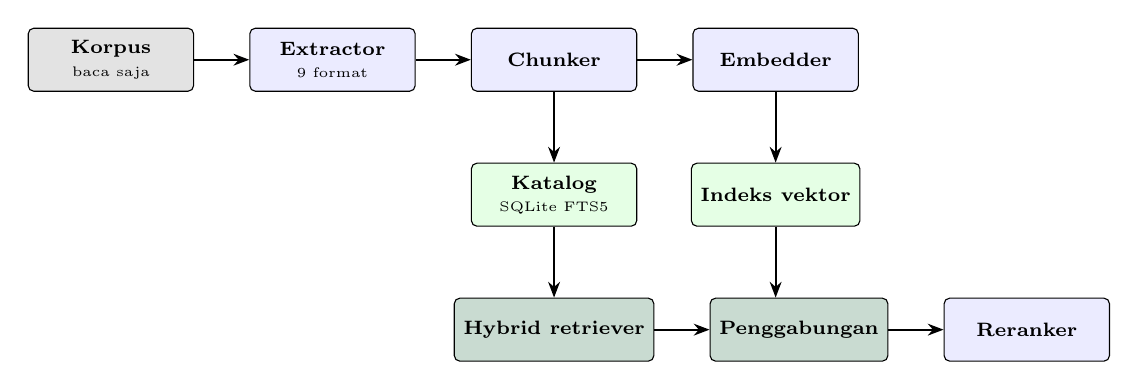
\begin{tikzpicture}[
      kotak/.style={draw, rounded corners=2pt, minimum width=2.1cm,
        minimum height=0.8cm, align=center, font=\scriptsize\bfseries},
      panah/.style={-{Stealth[length=2mm]}, thick}
    ]
      \node[kotak, fill=gray!22] (korpus) {Korpus\\
        {\tiny\mdseries baca saja}};
      \node[kotak, fill=blue!8, right=0.7cm of korpus] (ekstrak) {Extractor\\
        {\tiny\mdseries 9 format}};
      \node[kotak, fill=blue!8, right=0.7cm of ekstrak] (potong) {Chunker};
      \node[kotak, fill=blue!8, right=0.7cm of potong] (embed) {Embedder};

      \node[kotak, fill=green!10, below=0.9cm of potong] (katalog) {Katalog\\
        {\tiny\mdseries SQLite FTS5}};
      \node[kotak, fill=green!10, below=0.9cm of embed] (vektor) {Indeks vektor};

      \node[kotak, fill=praditagreen!25, below=0.9cm of katalog] (cari)
        {Hybrid retriever};
      \node[kotak, fill=praditagreen!25, right=0.7cm of cari] (gabung)
        {Penggabungan};
      \node[kotak, fill=blue!8, right=0.7cm of gabung] (tajam) {Reranker};

      \draw[panah] (korpus) -- (ekstrak);
      \draw[panah] (ekstrak) -- (potong);
      \draw[panah] (potong) -- (embed);
      \draw[panah] (potong) -- (katalog);
      \draw[panah] (embed) -- (vektor);
      \draw[panah] (katalog) -- (cari);
      \draw[panah] (vektor) -- (vektor|-gabung.north);
      \draw[panah] (cari) -- (gabung);
      \draw[panah] (gabung) -- (tajam);
    \end{tikzpicture}}

  \vspace{4pt}
  \raggedright
  {\small Baris atas mengisi indeks, baris bawah menjawab pertanyaan.}
\end{frame}

\begin{frame}{{\Large Gejala yang Sudah Terukur}}
  \vspace{6pt}
  {\small Keluaran \texttt{ukur\_kopling.py} atas repositori aslinya.}

  \vspace{6pt}
  \centering
  \small
  \begin{tabularx}{0.9\textwidth}{|l|r|r|r|}
    \hline
    \textbf{Modul} & \textbf{Baris} & \textbf{Fan-out} & \textbf{Fan-in} \\
    \hline
    \texttt{config} & 452 & 0 & 18 \\
    \hline
    \texttt{documents} & 249 & 0 & 8 \\
    \hline
    \texttt{safety} & 92 & 1 & 7 \\
    \hline
    \texttt{server} & 720 & 12 & 0 \\
    \hline
    \texttt{ingestion} & 747 & 7 & 1 \\
    \hline
  \end{tabularx}

  \vspace{6pt}
  \raggedright
  {\small \texttt{config} diimpor 18 modul dari 23 yang ada, sehingga
  perubahannya merambat. \texttt{server} mengimpor 12 modul, sehingga sulit
  diuji sendirian.}
\end{frame}

\begin{frame}{{\Large Biaya Menambah Satu Kemampuan}}
  \vspace{6pt}
  {\small Keluaran \texttt{ukur\_titik\_sentuh.py}. Titik sentuh adalah baris
  yang menyebut satu hal secara langsung.}

  \vspace{6pt}
  \centering
  \small
  \begin{tabularx}{0.9\textwidth}{|X|r|r|X|}
    \hline
    \textbf{Penambahan} & \textbf{Modul} & \textbf{Baris} & \textbf{Terbanyak} \\
    \hline
    Satu bahasa baru & 2 & 27 & \texttt{rag}, 26 baris \\
    \hline
    Satu negara baru & 8 & 72 & \texttt{query\_rewriting}, 30 baris \\
    \hline
  \end{tabularx}

  \vspace{6pt}
  \raggedright
  {\small Modul yang terlewat menjadi cacat yang baru terlihat saat dipakai.
  Angka inilah keadaan awal yang dibandingkan sesudah perubahan.}
\end{frame}

\begin{frame}{{\Large Memilih Fitur dan Dimensi}}
  \vspace{10pt}
  \begin{itemize}\small
    \item Pemilihan dimulai dari gejala yang terukur, bukan dari teknik yang
          sedang diminati.
    \item \textbf{\textit{Maintainability}} diukur dengan titik sentuh,
          \textit{fan-in}, \textit{fan-out}, dan berkas yang berubah.
    \item \textbf{Performa} diukur dengan median, persentil ke-95, dan nilai
          terbesar dari lama satu tahap.
    \item \textbf{Ketahanan} diukur dengan jumlah yang hilang, lama pulih, dan
          jumlah bagian yang ikut gagal.
  \end{itemize}

  \vspace{6pt}
  {\small Ketiganya dipilih sebab skripnya sudah tersedia, bukan sebab hanya
  ada tiga.}
\end{frame}

\begin{frame}{{\Large Sembilan Dimensi ISO/IEC 25010:2023}}
  \vspace{4pt}
  \centering
  \scriptsize
  \begin{tabularx}{0.97\textwidth}{|l|X|}
    \hline
    \textbf{Karakteristik} & \textbf{Contoh pada Exim} \\
    \hline
    \textit{Functional suitability} & Ketepatan sitasi terhadap potongan yang dikutip \\
    \hline
    \textit{Performance efficiency} & Latensi pencarian dan memori tiap unit \\
    \hline
    \textit{Compatibility} & Berjalan di atas mesin basis data lain \\
    \hline
    \textit{Interaction capability} & Biaya mengganti tema dan menambah bahasa \\
    \hline
    \textit{Reliability} & Jawaban tetap selesai ketika koneksi putus \\
    \hline
    \textit{Security} & Cakupan penjagaan sesi pada seluruh rute \\
    \hline
    \textit{Maintainability} & Titik sentuh, \textit{fan-in}, \textit{fan-out} \\
    \hline
    \textit{Flexibility} & Biaya menambah negara, bahasa, atau backend model \\
    \hline
    \textit{Safety} & Jaminan korpus tidak pernah berubah \\
    \hline
  \end{tabularx}

  \vspace{4pt}
  \raggedright
  {\small Daftar yang lebih luas dikenal sebagai \textit{ilities}, berguna
  mencari gagasan, namun definisi resminya tetap diambil dari ISO.}
\end{frame}

\begin{frame}{{\Large Menaikkan Peluang Diterima}}
  \vspace{8pt}
  {\small Makalah yang hanya melaporkan satu sistem yang diperbaiki jarang
  lolos pada jurnal bertingkat Q3. Objeknya tunggal, hasilnya dapat ditebak,
  dan artefaknya habis bersama naskahnya.}

  \vspace{6pt}
  \begin{itemize}\small
    \item \textbf{Menambah objek.} Ukuran yang sama dijalankan pada tiga
          sampai lima sistem lain. Paling murah, sebab skripnya berjalan pada
          paket Python mana pun.
    \item \textbf{Mengangkat ukurannya.} Yang diusulkan satu ukuran beserta
          alatnya, bukan perbaikan satu sistem.
    \item \textbf{Melaporkan \textit{trade-off}.} Kedua sisi berangka,
          misalnya \textit{maintainability} membaik sekian sedangkan latensi
          naik sekian.
  \end{itemize}

  \vspace{4pt}
  {\small Dengan cara pertama saja, Q4 masuk akal. Q3 menuntut cara pertama
  digabung salah satu cara lainnya.}
\end{frame}

\begin{frame}{{\Large Pilihan Judul: Maintainability}}
  \vspace{8pt}
  \begin{enumerate}\small
    \item \textit{From Hard-Coded Locales to a Language Registry} —
          \texttt{rag}, \texttt{server}.
    \item \textit{Adding a Country to a Regulatory RAG Corpus} —
          \texttt{crawl\_sites}, \texttt{query\_rewriting}.
    \item \textit{Plugin-Based Model Backends} — \texttt{language\_models}.
    \item \textit{Reducing Coupling of a Configuration Hub} — \texttt{config}.
    \item \textit{Splitting an HTTP God-Module} — \texttt{server}.
    \item \textit{The Extractor Registry as a Microkernel} —
          \texttt{extractors}.
  \end{enumerate}
\end{frame}

\begin{frame}{{\Large Pilihan Judul: Performa dan Ketahanan}}
  \vspace{8pt}
  \begin{enumerate}\small
    \setcounter{enumi}{6}
    \item \textit{Ports and Adapters for the Vector Index} — \texttt{storage}.
    \item \textit{Stage Reordering in a Hybrid Retrieval Pipeline} —
          \texttt{retrieval}.
    \item \textit{A Replicated In-Memory Index Across Query Units} —
          \texttt{storage}, Bab 8.
    \item \textit{Pipe-and-Filter Ingestion} — \texttt{ingestion}.
    \item \textit{Event-Driven Answer Streaming} —
          \texttt{answer\_streams}.
    \item \textit{Building a Read Model for Hybrid Retrieval} —
          \texttt{storage}, Bab 10.
    \item \textit{A Microkernel Core with Manifest-Declared Plugins} — tiga
          titik perluasan sekaligus.
  \end{enumerate}
\end{frame}

\begin{frame}{{\Large Pilihan Judul: Batas dan Pembagian}}
  \vspace{8pt}
  \begin{enumerate}\small
    \setcounter{enumi}{13}
    \item \textit{Does the Dependency Flow Really Go One Way?} — seluruh
          paket, Bab 2.
    \item \textit{Splitting Ingestion from Query Serving} —
          \texttt{ingestion}, \texttt{server}, Bab 11.
    \item \textit{Extracting the Crawler as a Deployable Service} —
          \texttt{crawler}, Bab 13.
    \item \textit{Swapping the Storage Engine Behind a Port} —
          \texttt{storage}, Bab 4.
    \item \textit{Theme Tokens Across Two Stylesheets} — \texttt{web/},
          Bab 3.
    \item \textit{Authentication as a Layer} — \texttt{server}, Bab 2.
    \item \textit{From Two Hard-Coded Roles to a Permission Registry} —
          \texttt{authentication}, Bab 4 dan 5.
  \end{enumerate}

  \vspace{4pt}
  {\small Kedua puluhnya hanya rekomendasi. Judul lain boleh diajukan.}
\end{frame}

\begin{frame}{{\Large Syarat Judul Usulan}}
  \vspace{10pt}
  \begin{itemize}\small
    \item Menunjuk modul yang benar-benar ada pada Exim.
    \item Menyebut teknik arsitektur dari bab sebelumnya.
    \item Menyebut dimensi kualitas yang diukur.
    \item Membawa dua \textit{research question} yang dapat dijawab dengan
          pengukuran.
  \end{itemize}

  \vspace{8pt}
  {\small Judul usulan dibicarakan lebih dahulu sebelum pekerjaannya dimulai,
  sebab judul yang ukurannya belum jelas akan menyulitkan seksi Metode
  Penelitian.}
\end{frame}

\begin{frame}{{\Large Pola Rancangan sebagai Alat}}
  \vspace{10pt}
  \begin{itemize}\small
    \item Gaya arsitektur menentukan bentuk besarnya, sedangkan pola
          menentukan cara memasangnya pada tingkat kelas.
    \item Pola disebut di seksi Desain Solusi sebagai cara, bukan di
          Pendahuluan sebagai sumbangan.
    \item \textit{Registry} dan \textit{Factory} untuk pendaftaran,
          \textit{Adapter} di belakang \textit{port}, \textit{Proxy} untuk
          \textit{cache}, \textit{Observer} untuk aliran peristiwa.
    \item Setiap lapisan tak langsung ada harganya, dan harga itu ikut
          dilaporkan.
  \end{itemize}
\end{frame}

\begin{frame}{{\Large Dua Research Question}}
  \vspace{6pt}
  {\small Pertanyaan yang baik menyebut apa yang diubah, apa yang diukur, dan
  pada keadaan mana.}

  \vspace{6pt}
  \centering
  \small
  \begin{tabularx}{0.95\textwidth}{|l|X|X|}
    \hline
    \textbf{Bentuk} & \textbf{Contoh} & \textbf{Buktinya} \\
    \hline
    Biaya perubahan & Berapa berkas berubah untuk menambah satu bahasa? & Keluaran skrip pada dua keadaan \\
    \hline
    Lama pekerjaan & Berapa median dan persentil ke-95 satu tahap? & Ratusan putaran pada beban sama \\
    \hline
    Ketahanan & Berapa bagian ikut gagal ketika satu gagal? & Kegagalan yang disisipkan \\
    \hline
  \end{tabularx}

  \vspace{6pt}
  \raggedright
  {\small "Apakah arsitektur ini lebih baik" tidak memenuhi syarat, sebab kata
  lebih baik tidak menyebut ukurannya.}
\end{frame}

\begin{frame}{{\Large Rancangan Pengukuran}}
  \vspace{8pt}
  \centering
  \resizebox{0.92\textwidth}{!}{%
    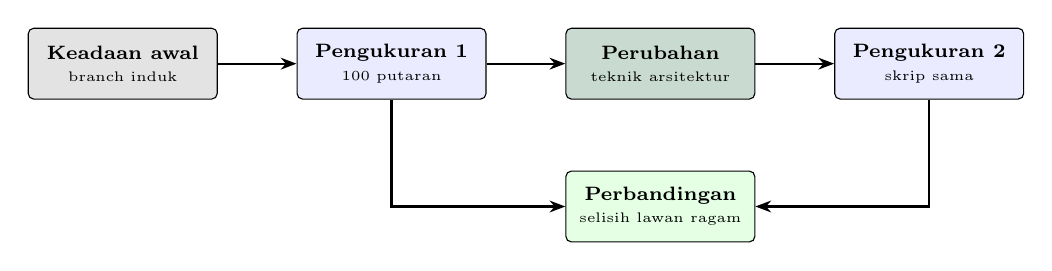
\begin{tikzpicture}[
      kotak/.style={draw, rounded corners=2pt, minimum width=2.4cm,
        minimum height=0.9cm, align=center, font=\scriptsize\bfseries},
      panah/.style={-{Stealth[length=2mm]}, thick}
    ]
      \node[kotak, fill=gray!22] (awal) {Keadaan awal\\
        {\tiny\mdseries branch induk}};
      \node[kotak, fill=blue!8, right=1.0cm of awal] (ukur1) {Pengukuran 1\\
        {\tiny\mdseries 100 putaran}};
      \node[kotak, fill=praditagreen!25, right=1.0cm of ukur1] (ubah)
        {Perubahan\\{\tiny\mdseries teknik arsitektur}};
      \node[kotak, fill=blue!8, right=1.0cm of ubah] (ukur2) {Pengukuran 2\\
        {\tiny\mdseries skrip sama}};
      \node[kotak, fill=green!10, below=0.9cm of ubah] (banding)
        {Perbandingan\\{\tiny\mdseries selisih lawan ragam}};

      \draw[panah] (awal) -- (ukur1);
      \draw[panah] (ukur1) -- (ubah);
      \draw[panah] (ubah) -- (ukur2);
      \draw[panah] (ukur1) |- (banding);
      \draw[panah] (ukur2) |- (banding);
    \end{tikzpicture}}

  \vspace{6pt}
  \raggedright
  {\small Skrip pengukurannya tidak boleh ikut diubah di antara kedua
  pengukuran.}
\end{frame}

\begin{frame}{{\Large Tiga Aturan Pengukuran}}
  \vspace{10pt}
  \begin{itemize}\small
    \item Satu kali pengukuran tidak cukup, sehingga tiap keadaan diulang
          sedikitnya seratus kali.
    \item Yang dilaporkan bukan rata-rata, melainkan median, persentil ke-95,
          dan nilai terbesar, sebab gejala antrean hanya terlihat pada nilai
          terbesar.
    \item Selisih yang lebih kecil daripada ragam antar putaran belum dapat
          disebut ada.
  \end{itemize}

  \vspace{8pt}
  {\small Pengukuran yang membaca kode tidak perlu diulang, tetapi definisinya
  wajib disebutkan, misalnya apakah komentar ikut dihitung.}
\end{frame}

\begin{frame}{{\Large Benchmark Pembanding}}
  \vspace{6pt}
  {\small Angka tidak bermakna bila berdiri sendiri, dan \textit{benchmark}
  ditetapkan sebelum pengukuran dimulai.}

  \vspace{6pt}
  \centering
  \small
  \begin{tabularx}{0.95\textwidth}{|l|X|}
    \hline
    \textbf{Jenis} & \textbf{Isinya} \\
    \hline
    Dasar & Keadaan awal sistem yang sama, mesin sama, beban sama. Wajib bagi seluruh judul \\
    \hline
    Tandingan & Cara lain yang sudah ada untuk pekerjaan yang sama, agar klaimnya tidak berputar pada diri sendiri \\
    \hline
    Batas & Biaya yang tetap dibayar meski pekerjaannya dihapus, menunjukkan ruang perbaikan yang tersisa \\
    \hline
  \end{tabularx}

  \vspace{6pt}
  \raggedright
  {\small Contoh batas dari Bab 8: antrean kosong melewatkan 1.200
  \textit{request} dalam 15,5 ms, sedangkan versi \textit{space} memakan
  65,6 ms.}
\end{frame}

\begin{frame}{{\Large Struktur Makalah}}
  \vspace{4pt}
  \centering
  \scriptsize
  \begin{tabularx}{0.97\textwidth}{|l|X|}
    \hline
    \textbf{Seksi} & \textbf{Isinya} \\
    \hline
    Pendahuluan & Latar belakang, celah, \textit{research question}, dan tujuan \\
    \hline
    Landasan Teori & Gaya arsitektur yang dipakai beserta istilahnya \\
    \hline
    Kajian Terkait & Pekerjaan orang lain beserta bedanya \\
    \hline
    Metode Penelitian & Rancangan, ukuran, dan cara tiap RQ dijawab \\
    \hline
    Desain Solusi & Susunan yang diusulkan beserta alasannya \\
    \hline
    Evaluasi & Lingkungan, beban, jumlah putaran, cara menghitung \\
    \hline
    Hasil & Angka apa adanya, tanpa penafsiran \\
    \hline
    Pembahasan & Penafsirannya, termasuk yang berlawanan dengan dugaan \\
    \hline
    \textit{Threats to Validity} & Ancaman kesahihan beserta cara menekannya \\
    \hline
    Kesimpulan dan \textit{Future Work} & Jawaban ringkas tiap RQ \\
    \hline
    Daftar Pustaka & Gaya IEEE \\
    \hline
  \end{tabularx}
\end{frame}

\begin{frame}{{\Large Aturan Template SAUCIS}}
  \vspace{6pt}
  \centering
  \small
  \begin{tabularx}{0.95\textwidth}{|l|X|}
    \hline
    \textbf{Hal} & \textbf{Aturannya} \\
    \hline
    Bahasa & Bahasa Inggris, naskah berbahasa lain ditolak \\
    \hline
    Berkas & Template LaTeX, sumber LaTeX wajib diunggah \\
    \hline
    Kemiripan & Di bawah 20 persen, tanpa daftar pustaka \\
    \hline
    Abstrak & Paling banyak 400 kata \\
    \hline
    Kata kunci & Tiga sampai lima, dipisah koma \\
    \hline
    Tabel & Keterangan di atas, gambar keterangan di bawah \\
    \hline
    Sitasi & Gaya IEEE, bernomor dalam kurung siku \\
    \hline
  \end{tabularx}

  \vspace{6pt}
  \raggedright
  {\small Naskah ditulis bahasa Indonesia dulu, lalu diterjemahkan sebelum
  dikirim. Kedua versi disimpan di \textit{branch} kelompok.}
\end{frame}

\begin{frame}[fragile]{{\Large Kerja Kelompok dan Branch}}
  \vspace{4pt}
\begin{lstlisting}[language=bash]
git clone https://github.com/alfa-yohannis/exim.git
git checkout -b capstone/<kelompok>-<judul-pendek>
# capstone/ukur/      skrip pengukuran dan keluarannya
# capstone/makalah/   naskah Indonesia dan terjemahannya
# capstone/README.md  judul, anggota, cara menjalankan
\end{lstlisting}

  \vspace{4pt}
  \begin{itemize}\small
    \item Pengukuran keadaan awal di-\textit{commit} sebelum perubahan kode
          dimulai, sehingga urutan waktunya terbukti dari riwayat.
    \item Keluaran pengukuran disimpan apa adanya, termasuk kejanggalannya.
    \item Dikumpulkan pada pertemuan terakhir, yaitu menurut jadwal Ujian
          Akhir Semester.
  \end{itemize}
\end{frame}

\begin{frame}{{\Large \textit{Summary}}}
  \vspace{10pt}
  \begin{itemize}\small
    \item Pada sistem yang sudah berjalan, yang dapat dipilih hanya bagian
          mana yang diperbaiki dan dengan teknik apa.
    \item Pemilihannya dimulai dari gejala yang terukur, misalnya
          \texttt{config} yang diimpor 18 modul dari 23.
    \item Dua \textit{research question} menentukan ukuran, isi Metode
          Penelitian, lalu urutan seksi Hasil.
    \item Arsitektur yang baik bukan yang terdengar rapi, melainkan yang
          perbaikannya dapat ditunjukkan dengan angka yang dapat dihitung
          ulang orang lain.
  \end{itemize}
\end{frame}

\end{document}
